\documentclass[../../thesis.tex]{subfiles}
\graphicspath{{\subfix{../../resources/}}}
\begin{document}

\section{Datasets}
The datasets used to evaluate the group sampling algorithm consist of real world
software systems and synthetically generated data.
We selected four software systems to be used to evaluate the group sampling algorithm on:
Apache HTTP Server, BerkeleyDB, PostgreSQL and JavaGC. All possible configurations of 
all four real-world datasets are already measured and thus are not subject to any variation
based on the testing environment. The real-world datasets are provided by the University of Leipzig.
Since we only look at binary features in this work, numerical
features are discretized into a number of mutually exclusive binary options \cite{siegmund2015performance}.
This lets us use a unified approach to both numeric and binary features of a
software system. 

In the following section a short overview of our four real-world examples is presented and
an explanation of how we generated our synthetic data.


\newpage

\begin{figure}[t]
    \begin{center}
        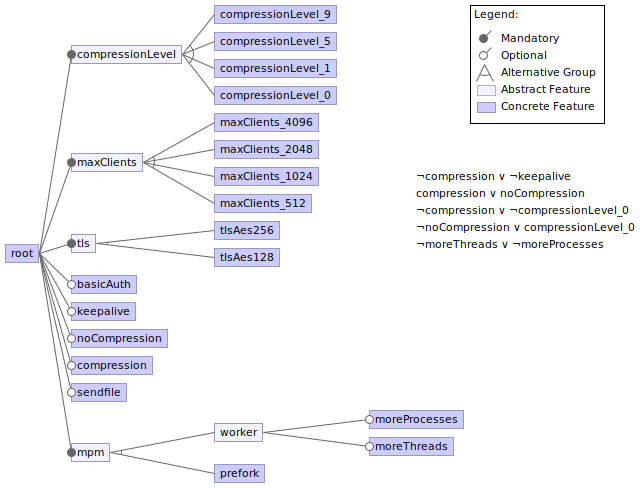
\includegraphics[scale=0.6]{./feature_diagrams/apache_feature_diagram.png}
    \end{center}
    \caption[Feature diagram - Apache HTTP Server]{Apache HTTP Server feature diagram - created with FeatureIDE}\label{fig:feature_diagram:apache}
\end{figure}

\paragraph{Apache}
The Apache HTTP Server is an open-source web server developed by the Apache Software Foundation
and is widely used today with a market share of 24.25\% in 2021 \cite{web:apachestatistic}.
The Apache dataset is the most restrictive of the real world datasets used
with 5 cross-tree constraints and 5 optional features not contained in an alternative group.
\\
\\
\begingroup
\renewcommand{\arraystretch}{1.5}
\begin{tabular}{lp{0.5\textwidth}}
    \textbf{Possible configurations:} & 13440                                 \\
    \textbf{Measured:}                & Performance                           \\
    \textbf{Influential features:}    & \textit{keepalive}                    \\
    \textbf{Independent features:}    & \textit{sendfile}, \textit{basicAuth} \\
\end{tabular}
\endgroup



\newpage
\begin{figure}[t]
    \begin{center}
        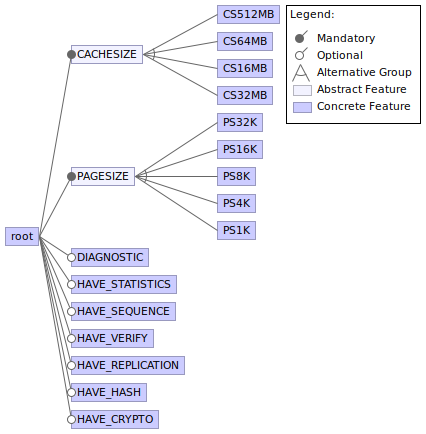
\includegraphics[scale=0.6]{./feature_diagrams/berkley_feature_diagram.png}
    \end{center}
    \caption[Feature diagram - BerkeleyDB]{BerkeleyDB feature diagram - created with FeatureIDE}\label{fig:feature_diagram:berkley}
\end{figure}
\paragraph{BerkeleyDB}
BerkeleyDB is an embedded database for key-value storage that originated at the University of California, Berkeley
and is now owned by Oracle \cite{web:berkeleydb}. The BerkeleyDB dataset is the simplest dataset used for the real-world examples with two numerical values
converted to an alternative group.
\\ \\
\begingroup
\renewcommand{\arraystretch}{1.5}
\begin{tabular}{lp{0.5\textwidth}}
    \textbf{Possible configurations:} & 2560                                                                                                                        \\
    \textbf{Measured:}                & Memory                                                                                                                      \\
    \textbf{Influential features:}    & \textit{PS32K}                                                                                                              \\
    \textbf{Independent features:}    & \textit{DIAGNOSTIC}, \textit{HAVE\_STATISTICS}, \textit{HAVE\_SEQUENCE}, \textit{HAVE\_VERIFY}, \textit{HAVE\_REPLICATION},
    \textit{HAVE\_HASH}, \textit{HAVE\_CRYPTO}                                                                                                                      \\
\end{tabular}
\endgroup


\newpage
\begin{figure}[t]
    \begin{center}
        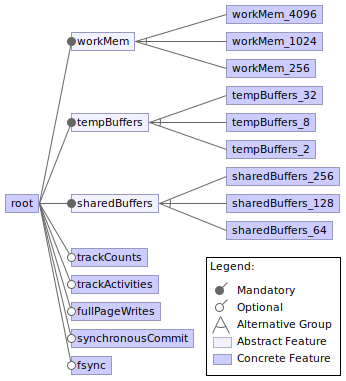
\includegraphics[scale=0.6]{./feature_diagrams/postgre_feature_diagram.png}
    \end{center}
    \caption[Feature diagram - PostgreSQL]{PostgreSQL feature diagram - created with FeatureIDE}\label{fig:feature_diagram:postgre}
\end{figure}
\paragraph{PostgreSQL}
PostgreSQL is an open-source database management system supporting extensible data types, operators, aggregations and functions \cite{web:postgresql}.
\\ \\
\begingroup
\renewcommand{\arraystretch}{1.5}
\begin{tabular}{lp{0.5\textwidth}}
    \textbf{Possible configurations:} & 19008                                                                                                               \\
    \textbf{Measured:}                & Performance                                                                                                         \\
    \textbf{Influential features:}    & \textit{fsync}                                                                                                      \\
    \textbf{Independent features:}    & \textit{trackCounts}, \textit{trackActivities}, \textit{fullPageWrites}, \textit{synchronousCommit}, \textit{fsync} \\
\end{tabular}
\endgroup



\newpage
\begin{figure}[t]
    \begin{center}
        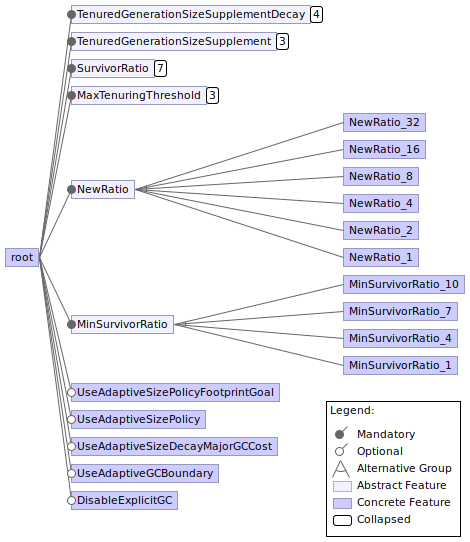
\includegraphics[scale=0.45]{./feature_diagrams/javagc_feature_diagram.png}
    \end{center}
    \caption[Feature diagram - JavaGC]{JavaGC feature diagram - created with FeatureIDE}\label{fig:feature_diagram:javagc}
\end{figure}
\paragraph{JavaGC} Java uses an automatic garbage collector (GC) to manage memory during the execution of a program.
It frees the memory of object which are no longer referenced and therefore no longer used.

In the feature diagram in \autoref{fig:feature_diagram:javagc} the features
\textit{TenuredGenerationSizeSupplementDecay}, \textit{TenuredGenerationSizeSupplement}, \textit{SurvivorRatio} and
\textit{MaxTenuringThreshold} are collapsed to make the diagram easier to read. All these values are discretized
numerical features.
\\
\begingroup
\renewcommand{\arraystretch}{1.5}
\begin{tabular}{lp{0.5\textwidth}}
    \textbf{Possible configurations:} & 193536                                                                                                                                                                            \\
    \textbf{Measured:}                & Performance                                                                                                                                                                       \\
    \textbf{Influential features:}    &                                                                                                                                                                                   \\
    \textbf{Feature interactions:}    & \textit{UseAdaptiveSizePolicy}, \textit{SurvivorRatio}, \textit{NewRatio}                                                                                                         \\
    \textbf{Independent features:}    & \textit{UseAdaptiveSizePolicy}, \textit{UseAdaptiveSizePolicyFootprintGoal}, \textit{UseAdaptiveSizeDecayMajorGCCost}, \textit{UseAdaptiveGCBoundary}, \textit{DisableExplicitGC} \\
\end{tabular}
\endgroup

\newpage

\subsection{Synthetic Data}

Our real-world examples consist of relatively small feature models with around 20 features.
Big software systems like the Linux kernel have more than 130,000 \cite{kaltenecker2020interplay} features.
To evaluate how the group sampling algorithm performs with a large dataset, we construct synthetic data
to freely control the properties the feature model has. These let us use more easily determine the
strength and weaknesses of our group sampling algorithm.

To generate the dataset, we specify the number of features, the number of constraints, the number of
alternative groups and the number of influential features. The constraints are generated by
randomly picking features and adding a random constraint between them. Either making them
mutually exclusive or letting the first feature imply the second one.
To add alternative groups to the feature model, we randomly pick a feature serving as the parent
of the alternative group and add constraints among a random amount of the following features to make them
mutually exclusive.

To make pseudo measurements on our feature model, each feature gets a weighting assigned to it.
We then randomly pick the specified amount of influential features and assign each non-influential feature
a random weighting from -5 to 5. The influential features are assigned a random weighting from
50 to 150. This lets us simulate the measurement of our generated feature model
by calculating the sum of all weights of the selected features. We also add a base value
of 200, to avoid getting negative simulated measurements.

We prepared three datasets for our evaluation.
The first, which we will call \textit{syn-100} contains 100 features, with four alternative groups, five random
constraints and one influential feature. The second, \textit{syn-500}, with 500 features, five alternative groups,
ten constraints and one influential parameter. And the third one, \textit{syn-1000}, with 1000 features, 10 alternative groups,
50 random constraints and two influential parameters.

We also prepared 4 datasets to test the group sampling on datasets with feature interactions. 
\textit{SYN-10-Interactions}, \textit{SYN-10-2-Interactions} with 10 feautres, one interaction and one influential feature.
And, two bigger datasets \textit{SYN-50-Interactions} and \textit{SYN-50-2-Interactions} where \textit{SYN-50-Interactions}
has 50 features, one influential and one interaction and \textit{SYN-50-2-Interactions} has 50 features, one influential and four interactions.

\newpage
\end{document}